\chapter{Formalization and Problem Analysis}
\label{ch:problem-analysis}

\section{Theoretical Foundation of Text Classification}

\label{sec:formalization}
For the sake of clarity it is useful to establish a framework of terminology and
notations that will be used in later explanations and in the course of
the entire master thesis. The notations introduced in this section can be
overviewed in table \ref{tab:notations}.

\subsection{Documents and Vocabulary}
The main goal of TC is to predict the category of pieces of textual data, also
called \emph{documents}.
Formally a document $d \in D$ is a tuple with $|d|$ elements such that
$d = (w_1,\ldots,w_{|d|})$, where $w_j, j=1,\ldots,|d|$ are the \emph{words}
contained in a document.
The meanings of the terms ``word'' and ``document'' don't necessarily coincide
with their colloquial counterpart. A ``word'' can also be a sequence of numbers
and/or symbols, a phrase ($N$-Gram) and a syntactically or a semantically tagged
word (see Section \ref{sec:complex-ling-feat}). A ``document'' $d$ is simply an
ordered collection of ``words''. 
Therefore, whenever this work refers to ``words in a document'', instead of
meaning ``word'' in the sense of a lexically valid word, we mean the elements
of a $|d|$-tuple $d$. For a shorter notation, when we want to
reference the $j$-th word of a document $d=(w_1,\ldots,w_{|d|}) \in D$ we will
write

\begin{equation*}
d^{(j)} = w_j, j=1,\ldots, |d|
\end{equation*}

We also introduce the \emph{domain of documents} $\mathcal{D}$ and the
\emph{domain of words} $\mathcal{V}$, that define the infinite sets of all possible
documents and all possible words respecitively, i.e. $D \subset \mathcal{D}$ and $V \subset
\mathcal{V}$.

For a set of documents $D=\{d_1,\ldots,d_{|D|}\}$ we also define the
a function that extracts all words contained in the documents of the dataset:
\begin{equation*}
\begin{split}
\mli{voc}&: \mathcal{P}(\mathcal{D}) \to \mathcal{P}(\mathcal{V}) \\
\mli{voc}&(D) = \left\{d(j) \mid d \in D, j =
1,\ldots,|d|\right\}
\end{split}
\end{equation*}

The set $V=\mli{voc}(D)$ is also called the vocabulary of $D$.
Analogously the vocabulary of a single documents is denoted as

\begin{equation*}
\mli{voc}(d) \coloneqq \mli{voc}(\{d\})
\end{equation*}

\subsection{Labels}

Let $\Omega=\left\{\omega_1, \omega_2,\ldots,\omega_{|\Omega|}\right\}$ be the
set of classes defined for the current classification problem. A document set
$D$ is called a \emph{labeled dataset} if there is a function $\omega: D \to
\Omega$, that assigns a labeled to each document $d \in D$. We call the function
$\omega$ a \emph{labelling over} $D$. If not specified otherwise, a dataset
identified with $D$ is a labeled dataset with labelling $\omega$.
On the other hand, \emph{unlabeled documents} or \emph{unknown documents} are
the the documents $\tilde{d} \in \mathcal{D}\setminus D$. 

The labelling $\omega$ is usually predefined by a domain expert
that manually preclassified the documents.
It is important to note that in this work each document has exactly one and only
one class associated to it. The subset of documents in a class $\omega \in
\Omega$ is denoted as:

\begin{equation*}
\begin{split}
D_\omega &\coloneqq  \{ d \mid \omega(d) = \omega\}, \omega \in \Omega \\
\end{split}
\end{equation*}

In the scope of this work, we will only consider the case of
\emph{binary classification}, i.e. the label of a document is either ``$+$''
(positive) or ``$-$'' (negative), i.e.  $\Omega = \{-,+\}$. \footnote{Multi-label
and multi-class problems --- i.e. the situations in which there multiple labels
for a document or more than two classes respectively --- can be handled by
solving several binary classification problems.}

\subsection{Word Frequencies}

Let $N_{v,d}$ be the amount of occurences of word $v \in \mathcal{V}$ in a
document $d$, i.e.

\begin{equation*}
N_{v,d} \coloneqq \sum\limits_{j=1}^{|d|} \mathbb{1}\{d^{(j)} = v\} \\
\end{equation*}

where $\mathbb{1}\{\cdot\}$ denotes the characteristic function.

Also, let $N_{v,\omega}^D$ refer to the number of occurences of word $v$ 
in documents $d \in D$ with label $\omega(d) = \omega$:

\begin{equation*}
N_{v,\omega}^D \coloneqq \sum\limits_{d \in D_\omega} N_{v,d}
\end{equation*}

The total amount of occurences of $v$ in a dataset $D$ is denoted as 

\begin{equation*}
	N_v^D = \sum\limits_{d \in D} N_{v,d}
\end{equation*}

\subsection{Statistical text classification}
\label{sec:statistical-tc}

\subsubsection{Bag-of-Words Model}
A common state-of-the-art method in text classification, is to use the
statistics yielded by words frequencies to predict the class of a document.
This implies transforming the textual data in a numerical representation
containing statistical information on the word frequencies in a labeled dataset.
One of the most used statistical document representations in text classification is the so called
\emph{Bag-of-Words (BoW)} [citation needed].
A document $d$ can be represented as a BoW in the following way

\begin{equation*}
\begin{split}
V = \left\{ v_1, \ldots, v_{|V|} \right\} \subset \mathcal{V} \\
\mli{bow}(V): \mathcal{D} \to \mathbb{N}^{|V|} \eqqcolon \mathcal{B}_V \\
\mli{bow}(d; V) \coloneqq \left(N_{d,v_1},  \ldots,
N_{d,v_{|V|}})\right)^\intercal
\end{split}
\end{equation*}

In other words, a BoW is a vector of positive integers and zero, whose
dimensionality equals the size of the vocabulary $V$. The $j$-th element of the
BoW vector indicates the frequency of word $v_j \in V$ in document $d$. We use
$\mathcal{B}_V$ denote the feature space defined by a BoW over a vocabulary $V$.

A common variant of the Bag-of-Words is the binary Bag-Of-Words (bBow), which is
defined as follows:

\begin{equation*}
\begin{split}
 \mli{bbow} &: \mathcal{D} \to \{0,1\}^{|V|} \coloneqq \mathcal{B}_V^{b} \\
\mli{bbow}(d) &\coloneqq (\mathbb{1}\{b_1 > 0\},\ldots,\mathbb{1}\{b_{|V|} >
0\})\\
(b_1, \ldots, b_{|V|})^\intercal &\coloneqq \mli{bow(d; V)}
\end{split}
\end{equation*}

Instead of representing the frequency of each word, the $j$-th element of a bBoW
vector is $1$ if $v_j$ is present in the corresponding document and $0$
otherwise. The corresponding feature space is denoted as $\mathcal{B}_V^{b}$.

Generally, we speak of a BoW model when the order in which the words occur in a
document is neglected and instead only the presence or the frequency of word
occurences is modelled. Classification based on this model is widely spread in
TC applications [citation needed]. As a baseline to compare our results with, we
introduce two of the most used and successful classifiers in text classification that are based
on the BoW model, namely the Multinomial Naive Bayes Classifier [citation
needed] and the linear Suppor Vector Machine (SVM) with Naive Bayes features,
the latter of which was introduced in \cite{wang2012baselines}.

\subsubsection{Multinomial Naive Bayes Classification} The Multinomial Naive
Bayes (MNB) classifier is a probabilistic classifier that performs
classification by estimating the probability of a class given a document. 
By the \emph{Bayesian rule} this probability is:

\begin{equation}
\label{eq:nb-bayes-rule}
\Pr(\omega\given d) = \frac{\Pr(d\given\omega)Pr(\omega)}{\Pr(d)} =
\frac{\Pr(d\given\omega)Pr(\omega)}{\sum\limits_{\omega' \in \Omega} \Pr(d\given\omega') \Pr(\omega')}
\end{equation}

In Bayesian terminology the probabilities mentioned in the equation above
are called

\begin{equation*}
	\text{posterior} = \frac{\text{likelihood}\times\text{prior}}{\text{evidence}}
\end{equation*}

The likelihood $\Pr(d\given \omega)$ is given by the
probabilities of the words occuring in $d$:

\begin{equation}
\label{eq:likelihood-full}
\Pr(d\given\omega) = \Pr(d^{(1)},\ldots,d^{(|d|)}\given\omega)
\end{equation}

However, in Naive Bayes (NB) models the ``naive'' assumption is made that word
occurences are conditionally indpendent, i.e. it is assumed that

\begin{equation*}
\label{eq:naive-bayes-assumption}
\Pr(d^{(1)},\ldots,d^{(|d|)}\given\omega) = \prod\limits_{i=1}^{|d|}
\Pr(d^{(i)} \given \omega)
\end{equation*}

Despite this assumption being wrong, NB models perform suprisingly
well in many classification tasks. A proof of why this is
the case can be found in \cite{zhang2004optimality}.

In MNB learning, the probabilities in equation \ref{eq:nb-bayes-rule} are
estimated using observations yielded by labeled dataset $D$. 
An estimate for the prior $\Pr(\omega)$ is given by the
relative frequency of positive/negative samples over the total amount of
samples in the labeled dataset:

\begin{equation}
\label{eq:priors}
\hat{P}(\omega) = \frac{|D_\omega|}{|D|}
\end{equation}

The likelihood of the model is approximated by the following term:

\begin{equation}
\label{eq:estimate-word-prob}
\hat{P}(v \given \omega) \coloneqq \frac{1+\sum\limits_{d \in
D_\omega}N(v,d)}{|V| + \sum\limits_{k=1}^{|V|} \sum\limits_{d' \in D_\omega}
N(v_k,d')} = \frac{1 + N(v,\omega)}{|V| + \sum\limits_{v' \in V} N(v', \omega)}
\end{equation}

In the equation above, estimates of the word probabilities are given by the
total count of a word in class $\omega$ (numerator) divided by the counts of all
words in that class (denominator). The summands $1$ in the numerator and $|V|$
in the denominator, are added to avoid zero- probabilities, in case a word
doesn't appear in $\omega$. This is also called \emph{Laplacian Smoothing}. The
rationale behind smoothing is that even when words do not appear in a
class $\omega'$, their true probability $\Pr(v \given \omega)$ is in fact
greater than 0.
Estimating the probability of a word to be zero is an underestimate, which
Laplacian smoothing compensates by slightly overestimating the word probabilties. 
[citation needed]

Using equations \ref{eq:estimate-word-prob} and \ref{eq:priors} and the naive
bayes assumption \ref{eq:naive-bayes-assumption} we can estimate the posterior
probability $\Pr(d \given \omega)$:

\begin{equation}
\begin{split}
\hat{P}(\omega \given d) \propto \hat{P}(\omega)\hat{P}(d\given \omega)
&= P(\omega)\prod\limits_{j=1}^{|d|} P(d(j) \given \omega) \\ &\eqqcolon
\ell(d,\omega)
\end{split}
\end{equation}

Note, that is equivalent to estimating the probability of a bag-of-words vector
if we assume that the features are all conditionally independent from each other:

\begin{equation}
\begin{split}
\textbf{b} \coloneqq \mli{bow}(d) &= (b_1, b_2, \ldots, b_{|V|}) \\ 
\hat{P}(\omega)\hat{P}(d\given \omega) = \hat{P}(\omega)\hat{P}(\mathbf{b}
\given \omega) &= \hat{P}(\omega)\hat{P}(b_1,\ldots,b_{|V|} \given
\omega)\\
&= \hat{P}(\omega)\prod\limits_{i=1}^{|V|}P(v_i|\omega)^{ b_i }
\end{split}
\end{equation}

A Naive Bayes \emph{classifier} is a function $c_{nb}$ that assigns a document the
class whose term $\ell(d, \omega)$ is larger, i.e

\begin{equation}
\begin{split}
c_{nb}&: \mathcal{D} \to \{+,-\} \\
c_{nb}(d) &= \begin{cases} + & \text{if~} \ell(d,+) > \ell(d,-) \\ - &
\text{if~} \ell(d,-) > \ell(d,+) \\ \text{rand}(\{+,-\}) &
\text{if~} \ell(d,+) = \ell(d,-)\end{cases}
\end{split}
\end{equation}

Note that since the eveidence $\Pr(d)$ (see Equation
\ref{eq:nb-bayes-rule}) does not depend on the class $\omega$, it is enough to
compute the term $\ell(d,\omega)$ to establish which posterior probability is
larger. In case that both classes are equally probable (third case), a class is
chosen randomly. 

\subsubsection{Linear SVM with Naive Bayes features}

In \cite{wang2012baselines} Wang et al. introduced the linear SVM with Naive
Bayes features (NB-SVM). In this section, we simply give a summary of the
findings reported in \cite{wang2012baselines}. For a more detailed description
of the rationales behind the design of the NB-SVM and for SVMs in general see
[citations needed].

As opposed to the standard approach of using a linear SVM to
classify documents in the feature space of BoWs [citation needed], they propose
to use the log-ratios of word frequencies as feature vectors. 
For a document $d$ in a labeled dataset $D$ with vocabulary $V = voc(D) = \{v_1, \ldots, v_{|V|} \}$ and classes
$\Omega = {+, -}$ this is:

\begin{equation*}
\begin{split}
\mathbf{p}(d) &\coloneqq \left(\mathbb{1}\{N_{v_1,+} > 0\} + \alpha, \ldots,
\mathbb{1}\{N_{v_{|V|},+} > 1\} + \alpha\right)^\intercal
\\
\mathbf{q}(d) &\coloneqq \left(\mathbb{1}\{N_{v_1,-} >0 \} + \alpha, \ldots,
\mathbb{1}\{N_{v_{|V|},-} > 0\} + \alpha\right)^\intercal \\
\mathbf{r}(d) &\coloneqq \log\left(\frac{\mathbf{p}(d) / \lVert
\mathbf{p}(d)\rVert_1}{\mathbf{q}(d) / \lVert \mathbf{q}(d)\rVert_1}\right) \\
\mathbf{f}(d) &\coloneqq \mathbf{r}(d) \circ \mli{bbow}(d; V)
\end{split}
\end{equation*}

Here $\alpha$ denotes a Laplacian Smoothing parameter and $\circ$ denotes the
elmentwise vector multiplication.  
The vector representation $\mathbf{f}(d)$ of a document is used to train the
weights $\mathbf{w}$ and the bias $b$ on a $L2$-regularized SVM by minimizing the following expression

\begin{equation}
\begin{split}
\mathbf{w}^\intercal\mathbf{w} + C\sum\limits_{d\in D} \max\left(0,
1-y(d)(\mathbf{w}^\intercal\mathbf{f}(d) + b)\right)^2 \\
y(d) \coloneqq \begin{cases} +1 & \text{if~} \omega(d) = + \\ -1 & \text{if~}
\omega(d) = - \end{cases}
\end{split}
\end{equation}

For the final model the weights are regularized using a parameter
$\beta \in [0,1]$:

\begin{equation*}
\mathbf{w'} = (1-\beta)\tilde{w} + \beta\mathbf{w}
\end{equation*}

where $\tilde{w} = \lVert \mathbf{w} \rVert_1/\lvert V \rvert$ denotes the
magnitude of $\mathbf{w}$.

A classifier based on this model is a function $c_{nbsvm}$ defined as follows:

\begin{equation*}
\begin{split}
\hat{y} &: \mathcal{D} \to \{+1,-1\} \\
\hat{y}(d) &= \sign(\mathbf{w'}^\intercal \mathbf{f}(d) + b) \\
c_{nbsvm} &: \mathcal{D} \to \{+,-\} \\
c_{nbsvm}(d) &= \begin{cases} + & \text{if~} \hat{y}(d) = +1 \\ - & \text{if~}
\hat{y}(d) = -1 \\ \mli{rand}(\{+, -\}) & \text{if~} \hat{y} = 0\end{cases}
\end{split}
\end{equation*}

The classification decision is taken based on whether a vector $\mathbf{f}(d)$
is on the left ($\hat{y}(d) = -1$) or on the right ($\hat{y}(d) = +1$) of the
plane defined by the normal vector $\mathbf{w'}$ and the bias $b$. For the
parameters $\alpha, \beta$ Wang et al. propose $\alpha = 1$ and $\beta =
\nicefrac{1}{4}$.
They perform experiments on various datasets using BoW representations
of unigrams and bigrams (see Section \ref{sec:complex-ling-feat}) and
experimentally show that the NB-SVM performs better than the Naive Bayes classifier and the standard linear SVM trained on bBoW features.

\subsection{Word Embeddings}

\subsubsection{Word2Vec}
Word embeddings are a more recent approach to represent words as numerical
vectors. In \cite{mikolov2013distributed} Milokov et al. introduced
\textit{Word2Vec}. They propose to generate word vectors with a shallow learning
network that estimates the probability $\Pr(w_O\given w_I)$ of an output word
$w_O$ given its context $w_I$. The context $w_I$ is defined by the words
surrounding $w_O$ within a symmetrical window size $k$. This is done by scanning
the training corpus in blocks of contiguous sequences of $2k + 1$ words and
using the middle word as input $w_I$ and the surrounding words as $w_O$. The network is trained in an 
unsupervised fashion by using a possibly large and topically heterogeneous text
corpus, e.g. the first billion words of \emph{Wikipedia} [citation needed].

The result of the training is a word embedding $\mathcal{W}=\left(V_{\mathcal{W}}, (\mathbf{x}_\mathcal{W}^{(i)})\right)$ 
with vocabulary $V_{\mathcal{W}} = \left\{ v_{\mathcal{W}}^{(1)}, \ldots,
v_\mathcal{W}^{(|V_\mathcal{W}|)} \right\} $ and corresponding word vectors
$x_\mathcal{W}^{(i)} \in \mathbb{R}^d, i=1,\ldots, |V_{\mathcal{W}}|$, each of
which represents a word $v \in V_\mathcal{W}$ in a $d$-dimensional real-valued vector space. Note that the dimensionality of the vector space is chosen as a parameter prior to the training process. An often
used and empirically well working dimensionality seems to be $d=300$ [citation
needed].
We denote the vector representation of a word in the vocabulary of the word
embedding as follows:

\begin{equation*}
\begin{split}
\mli{vec}: V_\mathcal{W} \to \mathbb{R}^d \\
\mli{vec}(v^i_{\mathcal{W}}) = \mathbf{x}_i
\end{split}
\end{equation*}

\subsubsection{Linguistic properties}
As reported in \cite{mikolov2013distributed} the vector representations
of words can be used to measure the semantic similarity between words. This can
be done by computing the angle between two word vectors:

\begin{gather*}
\mli{\text{cos-sim}}: \mathbb{R}^d \times \mathbb{R}^d \to [-1, 1] \\
\mli{\text{cos-sim}}(\mathbf{x}_1, \mathbf{x}_2) =
\frac{\mathbf{x}_1^\intercal\mathbf{x}_2}{\norm{\mathbf{x}_1}_2 \cdot
\norm{\mathbf{x}_2}}_2 = \cos \angle (\mathbf{x}_1, \mathbf{x}_2)
\end{gather*}

This measure is referred to as \emph{cosine similarity}, since it is
equivalent to calculating the cosine of the angle between two vectors. In the
embedding word vector space it, ranges from $-1$ (unrelated words) to $1$
(identical words). Table \ref{tbl:word2vec-examples} shows the cosine
distances for some word pairs. The distances were computed with word vectors
from the pretrained word embeddings model provided by google. It is noteworhty
that the words ``hot'' and ``cold'' are very close to each other, even though
they are antonyms. This is due to the fact, that words are mapped close to each
in the embedding vector space, if they are used in similar contexts. Therefore,
the semantic similarity yielded by word embeddings is more of a topical nature.

\subsubsection{Word distance measure}
A measure for word \emph{dissimilarity} can be expressed by
using the \emph{cosine distance}:

\begin{gather*}
\mli{\text{cos-dist}}: \mathbb{R}^d \times \mathbb{R}^d \to [0, 2] \\
\mli{\text{cos-dist}} \equiv 1 - \mli{\text{cos-sim}}
\end{gather*}

Note that strictly speaking, the cosine distance is not
a \emph{metric} since it does not satisfy the \emph{triangle
inequality}, i.e.

\begin{equation*}
\exists \mathbf{x},\mathbf{y},\mathbf{z} \in \mathbb{R}^d:
\mli{\text{cos-dist}}(\mathbf{x},\mathbf{z}) \not\leq
\mli{\text{cos-dist}}(\mathbf{x},\mathbf{y}) +
\mli{\text{cos-dist}}(\mathbf{y},\mathbf{z})
\end{equation*}

However, whenever this work refers to a \emph{distance} with respect to
words or word vectors, we refer to a measure that expresses their dissimilarity
such as the just introduced cosine distance.

For an embedding $\mathcal{W}=(V_{\mathcal{W}}, \mathbf{x}_i)$ we define the
following word distance measure:

\begin{equation*}
\begin{split}
\mli{dist}_\mathcal{W} &: \mathcal{V}\times \mathcal{V} \to [0,1] \\
\mli{dist}_\mathcal{W}(v,v') &= \begin{cases} 0 & \text{if~} v=v' \\
\frac{\mli{\text{cos-dist}}(vec(v),vec(v'))}{2} & \text{if~} v,v' \in
V_{\mathcal{W}}
\\
\infty & \text{if~} v \not\in V_{\mathcal{W}} \lor v' \not\in V_{\mathcal{W}}
\end{cases}
\end{split}
\end{equation*}

In the definition above we simply normalized the cosine distance to $[0,1]$,
which will be useful later in this work. Moreover, if one of the two words
is not covered by the word embeddings model, the distance function
returns an ``infinite'' distance. We use the symbol ``$\infty$''
to indicate a number that is greater than all real numbers, i.e. $\forall r
\in\mathbb{R}: r < \infty$. When both words are identical we
return the distance $0$, whether they are part of the word embeddings model or
not.

\begin{table}
\begin{tabular}{|l|l|l|}

\textbf{Notation} & \textbf{Description} & \textbf{Example} \\

$\mathcal{D}$ & set of all possible documents & \\
$\mathcal{V}$ & set of all possible words & \\
$D$ & set of preclassified documents & $D=\{ d_1, d_2\} = $\{('Hello', 'world'),
('Hello') \} \\

$D_\omega$ & set of documents of class $\omega$ & $D_+ = \left\{
\text{('Hello', 'world')} \right\}$ \\
& & $D_- = \left\{ \text{('Hello')} \right\}$ \\

$V = \mli{voc}(D)$ & vocabulary of $D$ & $V=$\{'Hello', 'world'\} \\
$\tilde{V}$ & OOV words $\mathcal{V} \setminus V$ &  \\
$N_{v,d}$ & counts of word $v$ in document $d$ & $N_{\text{'Hello'}, d_1} = 1,\
N_{\text{'world'}, d_2} = 0$
\\

$N_v^D$ & number of documents containing word $v$ & $N_{\text{'Hello'}}^D = 2$
\\

$N_{v,\omega}^D$ & counts of $v$ in $D_\omega$ & $N_{'world', -}^D = 0$ \\

$\mli{bow}(d; V)$ & BoW of document $d$ over vocabulary $V$ & $\mli{bow}(d_1; V)
= (1, 1)^\intercal,\ \mli{bow}(d_2; V) = (1,0)^\intercal$ \\

\end{tabular}
\caption{Formalization of \emph{TC}: Overview of Notations}
\label{tab:notations}
\end{table}

\subsection{Complex Linguistic Features}
\label{sec:complex-ling-feat}

\subsubsection{N-Grams}
\label{sssec:n-grams}
In BoW representations, the order in which words occur in a document is
neglected. Inspite of this, representing documents as BoWs has proven
to work reasonably well for many text classification tasks. A possible reason why this approach works, is
that the statistics of word occurences provide a good measure for predicting
the class of a document. E.g., the Naive Bayes classifier estimates the
posterior probability $\Pr(\omega\given d)$ of a class $\omega$ given a document $d$ by essentially counting the occurences 
of each word for each class (see Section \ref{sec:statistical-tc}).

However, the order in which words occur can often yield important information
that are relevant to the classification task. Consider the sentences ``no,
it's good" and ``it's no good" within a sentiment analysis task. Despite
expressing the opposite sentiment, in their BoW representation
with the vocabulary $V = \left\{\text{'no', 'it's', 'good'} \right\}$ 
the two sentences would be identical and thus impossible to distinguish for a
classifier that operates on Bag-Of-Words.

A technique that is commonly used to represent the local order
of words is to include \emph{$N$-grams}. In text classification, an $N$-gram is
a contiguous sequence of $N$ words from a given document. $N$-grams of size one are called
\emph{unigrams}, of size two \emph{bigrams}, and of size three \emph{trigrams}.
$N$-grams for $N > 3$ are referred to as four-grams, five-grams, six-grams, etc.

E.g., consider the following sentence:

\begin{center}
\textit{It's a beautiful day}
\end{center}

Here the unigrams are

\begin{center}
\begin{tabular}{|c|c|c|c|}
\hline
It's & a & beautiful & day \\
\hline
\end{tabular}
\end{center}

The bigrams are

\begin{center}
\begin{tabular}{|c|c|c|c|c|}
\hline
<s> It's & It's a & a beautiful & beautiful day & day </s> \\
\hline
\end{tabular}
\end{center}

where ``<s>'' and ``</s>'' are tokens that denote the start and the end of the
sentence respectively. 
A common approach to include $N$-grams in a dataset is
to concatenate each document with its $N$-grams as follows 

\begin{center}
\begin{tabular}{|c|c|c|c|c|c|c|c|c|}
\hline
It's & a & beautiful & day & <s> It's & It's a & a beautiful & beautiful day &

day </s> \\
\hline
\end{tabular}
\end{center}

We define the $N$-Grams represantion of a document for $N=n$ as follows:

\begin{equation*}
\begin{split}
g_n &:  \mathcal{D} \to \mathcal{D}, n \geq 2 \\
d &= (w_1,w_2,\ldots,w_{|d|}) \in \mathcal{D} \\
g_n(d) &=  (\underbrace{(S_0,w_1, \ldots,
w_n)}_{\mathrm{Tuple~of}~n\mathrm{~contiguos~words}}, \ldots,
(w_{|d|-n+2},\ldots,w_{|d|},S_1))
\end{split}
\end{equation*}

where $S_0, S_1$ are special tokens that define the start
and the end of a document respectively.

As in \cite{wang2012baselines, furnkranz1998study}, whenever we use $N$-grams of
size $N$ for text classification, a document is represented by concatenating it
with all representations of $k$-Grams with $k \leq N$. E.g., if we use trigrams, then the bigrams and the
unigrams are also included in the document representation. 
We define the operation of adding $N$-Grams up to a size $N$ to a
document as

\begin{equation*}
\begin{split}
g_N^* &: \mathcal{D} \to \mathcal{D}, N \geq 2 \\
g_N^*(d) &= d~\Vert~g_2(d)~\Vert \ldots \Vert~g_N(d) \\
g_N^*(D) &\coloneqq \left\{g_N^*(d_1),\ldots,g_N^*(d_{|D|})\right\}
\end{split}
\end{equation*}

where $||$ is the tuple-concatenation operator.

A representation as BoW \footnote{A BoW that represents N-Grams is also called a
\emph{Bag-Of-N-Grams}. } follows directly by applying $g_N^*$ to all documents
in a dataset $D$ and computing the word frequencies using the vocabulary
$V_N^* = \mli{voc}(g_N^*(D))$. We also define a partition of the vocabulary
$V_N^*$ over the different $N$-Gram sizes $n=1,\ldots,N$:

\begin{equation*}
\begin{split}
V_n &=  \left \{(d^{(i)},
d^{(k+1)},\ldots,d^{(k+n-1)}) \mid d \in D \wedge 1 \leq k \leq |d|-n+1
\right\} \\
& \cup \{ (S_0,d^{(1)},\ldots,d^{(k+N)})  \mid d \in D \} \\
& \cup \{ (d^{(|d|-N+2)},\ldots,d^{|d|},S_1) \mid d \in D\} \\
V_N^* &\coloneqq V \cup \bigcup\limits_{n=2}^N  V_n \\
\end{split}
\end{equation*}

\subsubsection{Part-Of-Speech Tagging}
Another approach to enrich BoW with additional information about the words
contained in a document, is to so called \emph{Part-Of-Speech (PoS) tagging}.
This refers to annotating each word with its grammatical function within the sentence it occurs.
For our example sentence this would look like

\begin{center}
\begin{tabular}{|l|l|}
\hline
\textbf{Word} & \textbf{PoS} \\
\hline
It 		  & \emph{pronoun} \\
's 		  & \emph{finite verb} \\
a 		  & \emph{indefinite article}  \\
beautiful & \emph{adjective} \\
day		  & \emph{noun} \\
\hline
\end{tabular}
\end{center}

Generally speaking, PoS-Tagging implies adding linguistic and
grammatical modifiers to tokens within a document:

\begin{equation*}
(v,m_1,m_2,\ldots,m_l) \in
V \times M_1 \times M_2 \times \ldots M_l
\end{equation*}
Which modifiers $M_j$ are used, depends on the implementation of the
PoS-Tagger and the document language. Possible modifiers include the word
type (noun, verb, adjective) to the morphological form (grammatical case,
grammatical gender, grammatical number) and the grammatical function
(subject, object, predicate) of the tagged word.

A document $d \in D$ is then preprocessed as follows by a PoS-Tagger:

\begin{equation*}
\begin{split}
\mli{pos} &:  \mathcal{D} \to \mathcal{D} \\
d &= (w_1,w_2,\ldots,w_{|d|}) \in \mathcal{D} \\
\mli{pos}(d) &=  \left((w_1\underbrace{,
m_1^1, \ldots,m_1^l}_{\mathrm{Modifiers}}), \ldots,
(w_{|d|},m_{|d|}^1,\ldots,m_{|d|}^l)\right) \\
\end{split}
\end{equation*}

$V_P$ denotes the set of token-modifiers tuples by which
the vocabulary is extended after the tagging process.

\begin{equation*}
V_P = \left\{ p_i^k \mid pos(d_i) = (p_1^i,\ldots,p_{|d|}^i), d_i \in D, 1 \leq
k \leq |d_i| \right\}
\end{equation*}
As with $N$-Grams, usually
the PoS-Tagged document is concantenated with original document and then
represented as BoW.

\section{Challenges in Text Classification}

The complexity and variability of human language makes text
classification a non-trivial task as it implies working in very high
dimensional feature spaces. Even for small datasets, with a few hundred of
samples, the BoW representation of a document can reach thousands of dimensions.
Adding complex linguistic features increases the dimensionality even more. The
problems resulting from high dimensional feature spaces are described in the
following sections.

\subsection{Unfrequent words and sparse Feature Vectors}

In \cite{wang2012baselines} Wang et al. experimentally showed that just by
affixing bigrams as described in Section \ref{sssec:n-grams}, classification
accuracies can be slightly improved.
Nonetheless, using $N$-\textit{grams} with $N > 2$ didn't make the
classification accuracy better.
One way to explain why this happens, is by considering how the
statistics of each $N$-gram are affected, when $N$ grows.

Assume a unigram $v$ appears $N_v$ times in a given dataset $D$. All bigrams
$(v,v')$ for $v' \neq v$ can't possibly occur more often than  $v$ itself.
Generally speaking $N_{(v,v')} \leq N_v$.
The same logic can be applied to $N$ and $N+1$ for $N >= 2$.\footnote{W.l.o.g.
this can also be said about bigrams $(v'',v)$ with $v '' \neq v$.} In the
extreme case, when $N = \max_{d' \in D} |d'|$, then every $N$-gram occurs at most one time. In short,
what we observe is that by building bigger and bigger $N$-grams the
Bag-Of-Words represantion of documents $d \in D$ becomes more sparse, i.e. in
proportion the number of zero-entries in a feature vector grows.

For count-based classifiers, this this might present a problem. In its
frequentist interpretation, the probability of an event, in this case that an
$N$-gram $v$ appears in class $\omega$, is approximated by
its relative frequency with respect to the counts of $v_k$ in the whole dataset:

\begin{equation*}
\Pr(v \given \omega) \approx \frac{1 + N(v,\omega)
}{|V| + \sum\limits_{v'\in V} N(v',\omega)} =:
\hat{P}(v \given \omega)
\end{equation*}

The main claim of frequentist probability theory is that for inifnite samples
the relative frequency converges to the true underlying probability, in the same
way as the relative frequency of throwing ``heads'' with a fair coin, will
approach 0.5 with a growing number of coin throws. Therefore, as we consider the
number of observed documents $|D|$ approaching infinity, we obtain

\begin{equation*}
\Pr(v \given \omega) = \lim_{|D| \to \infty} \frac{1 + N(v,\omega)
}{|V| + \sum\limits_{v'\in V} N(v',\omega)}
\end{equation*}

With fewer occurences for each $N$-gram, the estimates for the word probabilities
become more biased due to the scarcity of observations. This phenomenon is also
known as \emph{sampling error}. \footnote{If we assume a
gaussian distribution, then the sampling error $\epsilon \in
\mathcal{O}(1/\sqrt{|D|})$, which implies that in order to halve the error one
needs to enlarge the training set from $|D|$ to $|D|^2$ samples.} This error
propagates to the estimated posterior probability $\hat{P}(\omega|d)$.
The result is that words with low counts act like noise, which on average has no
impact on classification accuracy at all or can even worsen a classifier's
predictive ability. As a consequence, even though they contain more
information, arbitrarily adding higher order features such as $N$-grams or
PoS-tags cannot be expected to be generally beneficial to text classification
tasks. \footnote{What we here describe as statistical sparsity or sampling
error can be also viewed as a special case of the \emph{curse of
dimensionality}}

\subsection{Out of Vocabulary Words}
\label{ssec:oov}

Another challenge in text classification is \emph{Out-Of-Vocabulary
(OOV)} words. OOV words are encountered in the case in which an unknown document
$\tilde{d} = (\tilde{w}_1, \ldots, \tilde{w}_{|\tilde{d}|}) \in
\mathcal{D}\setminus D$ , i.e.
a document for which the true label is not known, contains words that are not
part of the classifier's known vocabulary.
As a consequence, the information provided by OOV words cannot be used for
prediction, since they do not have any representation in the classifier's feature
space. Formally these are the words

\begin{equation*}
\tilde{V} \coloneqq \mathcal{V} \setminus V
\end{equation*}

Note that, for the same reasons described in the previous section, when using
complex higher features, OOV-words become even more frequent.

\section{Case Study: Echobot}
\label{sec:echobot}

The detrimental effects of high dimensional feature spaces, make it difficult to
use enriched features such as $N$-Grams and $PoS$-Tags in small datasets.
An example of how these difficulties are overcome in a real-word scenarion
can be found at \textit{Echobot}, a small German company that develops machine
learning based tools for social media monitoring and sales.

\subsection{Company description}
Their goal is to offer their customers solutions that
help oversee what the web is reporting about their products, their firm or
their competitors, helping them to adjust their business strategy according
to trends detected on the web. Web content is retrieved by a complex web crawler
that scans millions of social media postings and hundreds of thousands
of articles and company websites daily. The information gathered in this way is
analyzed, structured and categorized with machine learning based software that
extracts useful and relevant information for the customer.

\subsection{Business Signals}

In one specific context, text classification is used to alert customers when
newly published web content concerns a specific topic. E.g., one might
be interested in knowing when a company of a specific industry is about to change
their management personell or has announced a site closure.
Events like this, also called \textit{business signals}, are of particular
commercial interest for the customer. For example, it is known that a
restructuring of a company's managing personell, is often followed by the purchase of new
services and products. With this knowledge at hand, a salesman that has been
alerted of such event, could contact the company in question and make an offer
before anyone else.

\subsection{Semi-Automated Text Classification}

When classifying business signals, Echobot faces the same problems
mentioned in the introductory chapter: labeled data is scarce and costly to produce,
but nonetheless crucial for effective text categorization. Therefore, in order
to optimize classification accuracy inspite of the scarcity of labeled data, Echobot developed
a semi-automated classification process that involves a human agent. Instead of
building a classification model based on the raw textual data, a domain expert
preprocesses the documents by annotating each sample with semantic and
syntactic information that will help the classifier build a more precise
classification model. As a matter of fact, the benefits of this method can be
observed experimentally: compared with its unpreprocessed variant, classification with
the annotated dataset performs significantly better. Therefore, an analysis of
how the domain expert preprocesses the datasets, might give an intuition for
an \emph{automated} preprocessing method that improves classification
effectiveness.

\subsection{Manual preprocessing by a domain expert}
 
The linguistic of the domain expert are leveraged for a twofold task:

\begin{itemize}
  \item The selection and combination of a pool of PoS-tags and $N$-grams and
  other complex linguistic features
  \item The creation of dictionaries of semantically related words that are used
  to for substituting words in the dataset
\end{itemize}

 
 

\subsubsection{Dictionary based word substitutions}

We can describe the operations of the domain expert formally as follows:
let $D$ be a set of documents containing $N$-grams $V_N^*$ and
PoS-Tags $V_P$ such that $V = V_N^* \cup V_P$.
The operator's task is to combine the available $N$-grams and PoS-Tags
such that the resulting feature space reflects his understanding
of semantics for the underlying classification task.
More formally, this implies the creation of a list of rules
$\boldsymbol{\rho} = (\rho_1, \rho_2, \ldots, \rho_n)$, where each rule $\rho_i:
\mathcal{B} \to \mathbb{N}$ for $i=1,2,3,\ldots,n$ maps a subspace of the BoW
feature space $\mathcal{B}$ to a scalar value.

\begin{eqnarray*}
\mathcal{H} \coloneqq \mathbb{N}^n \\
\boldsymbol\rho: \mathcal{B}_V \to \mathcal{H} \\
\boldsymbol{\rho}(\mathbf{b}) = (\rho_1(\mathbf{b}), \ldots,
\rho_n(\mathbf{b}))^\intercal
\end{eqnarray*}

In other words, after applying $\boldsymbol\rho$, the classification problem is
transfered from the large feature space of BoW's to a lower dimensional and
semantically enriched vector space engineered by the domain expert.

The following toy example illustrates how such a rule might look
like for a specific vocabulary:

\begin{equation*}
\begin{split}
V_P \supset \{(\text{'good', ADJ})\}, V_2 \supset \{(\text{``not"},
\text{``bad"})\}
\\
\rho_1(\mathbf{b}) = \mathbf{b}((\text{'good',ADJ})) +
\mathbf{b}((\text{``not", ``bad"}))
\end{split}
\end{equation*}

Here the notations $\mathbf{b}(v)$ indicate the entry of the Bag-of-Words
$\mathbf{b}$ for the word $v \in V$. The rule above additively combines the
occurences of the adjective ``good'' and the bigram ``not bad'' to one new
feature. The process is represented graphically in Figure \ref{fig:rho}.

%\usepackage{graphics}
% is needed for
% \includegraphics
\begin{figure}[htp]
\begin{center}
  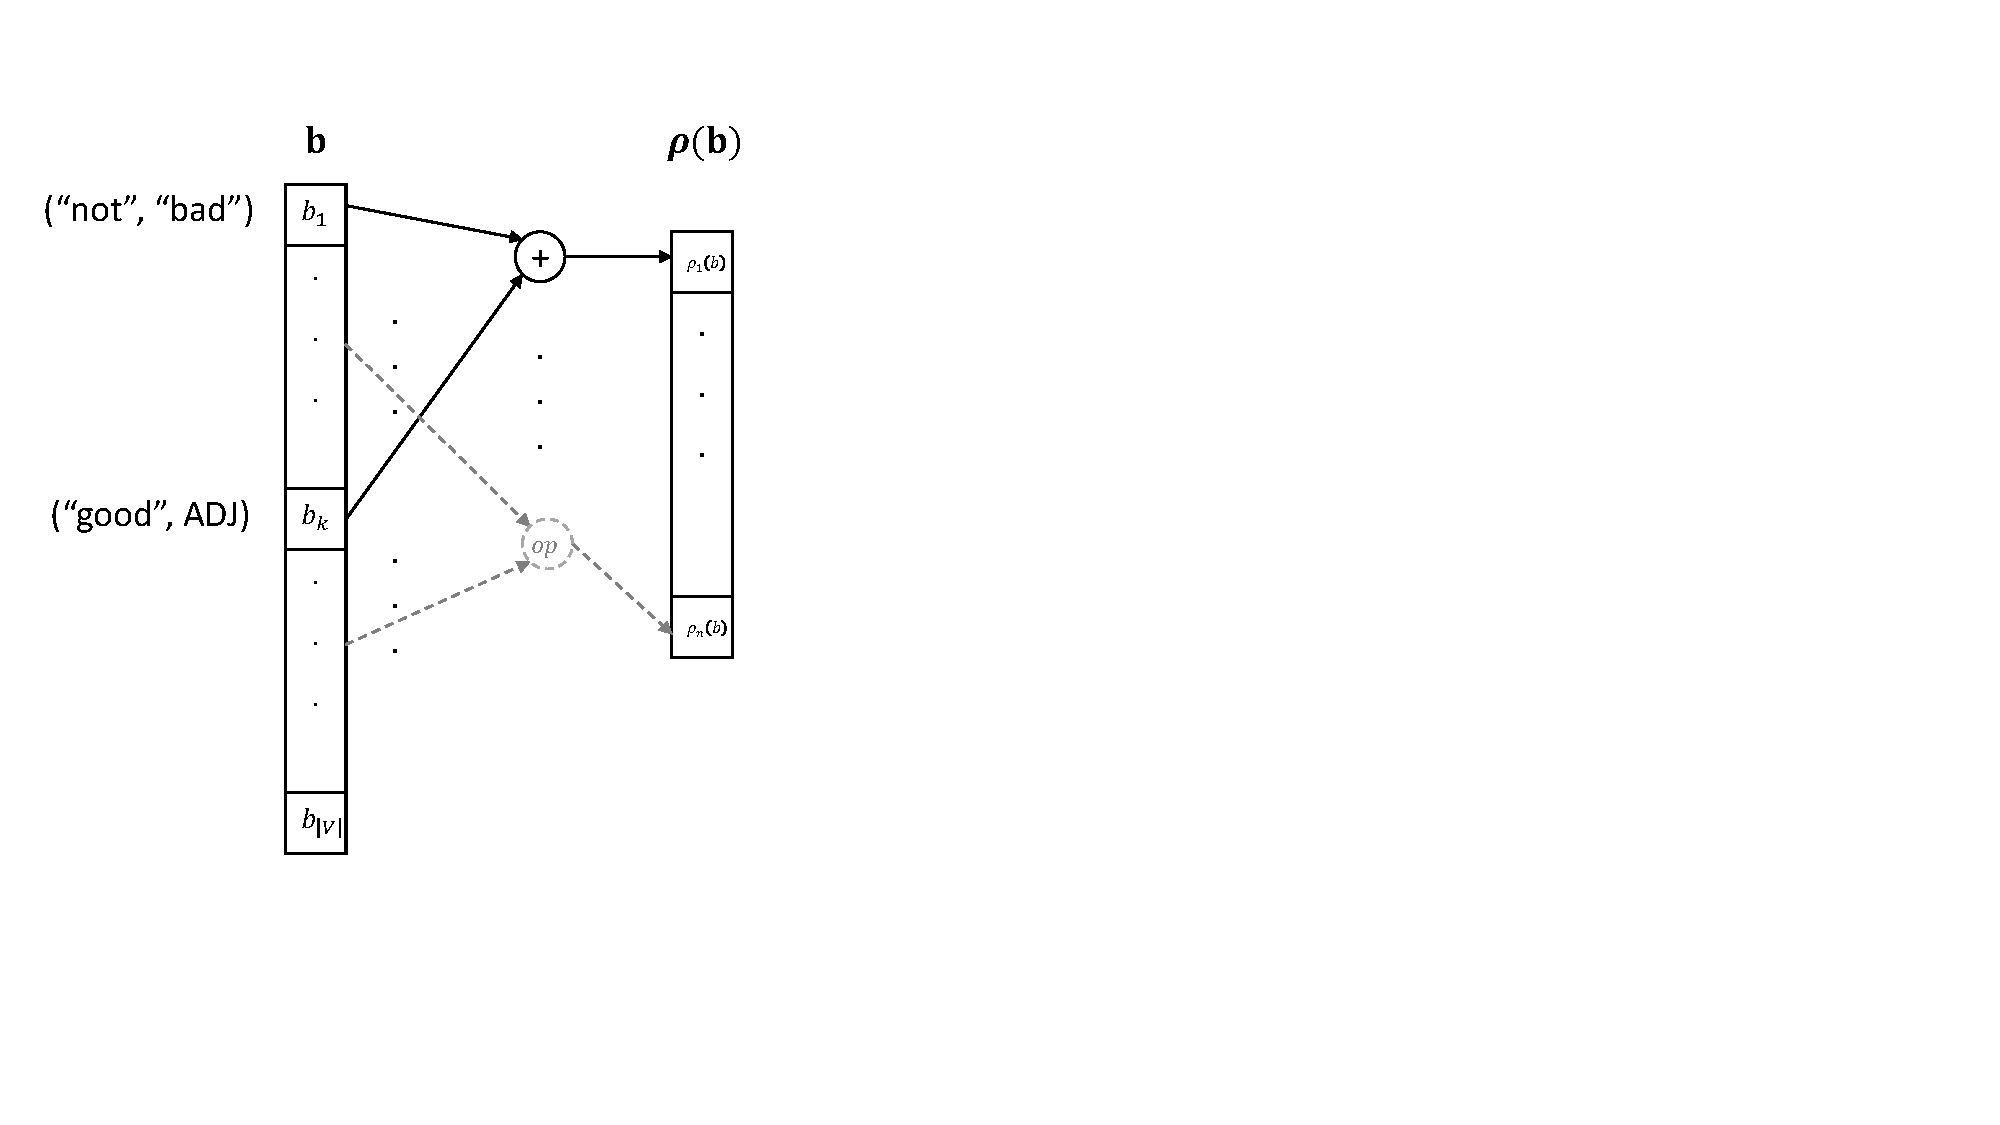
\includegraphics[trim= 0 45.94mm 210mm 21mm, clip, scale=0.5]{img/rho}
  \caption[Example for rule based features]{Example for rule based features:
  The BoW dimensions for ``not bad'' and ``good'' are combined in to a new
  feature by adding the frequencies of their occurences.}
  \label{fig:rho}
\end{center}
\end{figure}

In this example the utility of using complex linguistic features becomes
 clear: by using the PoS-Tag ``good", it is possible to disambiguate the
its meaning, e.g. from ``good'' as a synonym for ``product''. Moreover,
using the bigram ``not bad" allows to establish whether the word ``bad'' was
used in a negative or in a positive way. This cannot be achieved if the words ``not'' and ``bad'' are
represented separately as unigrams, as the word ``not'' could a
appear in a context that does not refer to ``bad''. The feature generated by
$\rho_1$ can be interpreted as a simple indicator for the polarity of a
sentence, which in a task of sentiment analysis would be useful to discriminate
positive from negative examples.

In order to handle OOV words, the domain expert preemptively creates a
set of synonyms to which the classifier can fall back to in case a word is not contained
in the known vocabulary. He thereby selects a subset of words $v^* \in V^*
\subset V$, that might be important for classification. Subsequently,
for each $v^* \in V^*$ a set $T_{v^*} \subset \mathcal{V}\setminus V$ of OOV
words, that are semantically similar to $v*$ is created.  Unknown samples $\tilde{d} \in D$ can then be
preprocessed as follows:

\begin{eqnarray*}
\tilde{d} := (\tilde{w_1},\ldots,\tilde{w}_{|\tilde{d}|}) \in
\mathcal{D}\setminus D
\\
\boldsymbol\pi: \mathcal{D} \to \mathcal{D} \\
\boldsymbol\pi(\tilde{d}) =
(\pi(\tilde{w_1}),\ldots,\pi(\tilde{w}_{|\tilde{d}|})) \\
\pi(\tilde{w}_k) = \begin{cases} \tilde{w}_k & \tilde{w}_k \in V  \\
v^* & \tilde{w}_k \in T_{v^*} \\
\mathrm{<unknown>} & \mathrm{otherwise} \end{cases}& ,~k=1,\ldots,|\tilde{d}|
\end{eqnarray*}

Where ``<unknown>'' is used as a token in case there is no alternative available
for an OOV word.
An example for such a list $T_{v*}$ would be the following:

\begin{equation*}
T_{\text{``good''}} = \{\text{``outstanding''}, \text{``excellent''}, \ldots\}
\end{equation*}

In this case, we the words ``outstanding'' and ``excellent'' do no
appear in the underlying dataset. If either word is seen in an unknown
document, it is mapped to the semantically related word ``good''.

\subsubsection{Benefits of word substitutions in text classification}

In section \ref{sec:challenges} we considered two of the main problems in TC
introduced by high dimensional feature spaces, especially when using higher
complex linguistic features such as N-Grams and PoS-tags, i.e. feature sparsity
and OOV-words. We now address the question of how the preprocessing done by the
domain in fact implies an alleviation of the mentioned problems .

\paragraph{Reduction of feature sparsity}
In order to show how rule based features can be helpful for text classification,
we are going to consider a polarity task that has be solved using Naive Bayes
learning on a toy dataset with the following word distributions:

\begin{center}
\begin{tabular}{|c|c|c|c|c}
$v$ & $N(v, +)$ & $N(v,-)$ & $\hat{P}(v\given +)$ & $\hat{P}(v \given -)$ \\
\hline
This & $23$ & $25$ & $2.4\cdot 10^{-3}$  & $2.6 \cdot 10^{-3}$\\
is & 45 & 47 & $4.6\cdot 10^{-3}$ &  $4.8\cdot 10^{-3}$ \\
good & 10 & 3 & $1.1 \cdot 10^{-3}$ & $4.0 \cdot 10^{-4}$ \\
not bad & 1 & 1 & $2.0 \cdot 10^{-4}$ & $2.0 \cdot 10^{-4}$   
\end{tabular}
\end{center}

The class conditional word probabilities with the method described in
section \ref{sec:naive-bayes}.In this example we chose the smoothing parameter
to be $\alpha = 1$.
Assume we want the task is use the estimations of a Naive Bayes model to
predict the polarity of the sentences ``This is good''($\eqqcolon d_i$) and
``This is not bad'' ($\eqqcolon d_2$).
which are represented, whos true label we assume to be $\omega(d_1) =
\omega(d_2) = +$. The sentences are represented by the following tuples:

\begin{equation*}
\begin{split}
d_1 = (\text{'This'}, \text{'is'}, \text{'good'}) \\
d_2 = (\text{'This'}, \text{'is'}, (\text{'not'}, \text{'bad'}))
\end{split}
\end{equation*}
If we assume prior class probabilities $\hat{P}(+) = \hat{P}(-) = 0.5$,
then the estimated a posteriori probabilities of $d_1$ are the following:

\begin{equation*}
\begin{split}
\hat{P}(d_1|+) &=  \hat{P}(\text{'This'} \given +) \cdot \hat{P}(\text{'is'} \given +) \cdot \hat{P}(\text{'good'} \given
+)\\ &= 11.9 \% \\
\hat{P}(d_1|-) &=  \hat{P}(\text{'This'} \given -) \cdot \hat{P}(\text{'is'} \given -) \cdot \hat{P}(\text{'good'} \given
-) \\ &= 4.9 \% \\
\\
\hat{P}(+|d_1) &= \frac{\hat{P}(d_1 \given +)\cdot \hat{P}(+)}{\sum\limits_{\omega' \in \{+,-\}}
\hat{P}(d_1 | \omega')} = 70.9 \% \\
\hat{P}(-|d_1) &= \frac{\hat{P}(d_1 \given -)\cdot
\hat{P}(-)}{\sum\limits_{\omega' \in \{+,-\}} \hat{P}(d_1 | \omega')} = 29.1 \%
\end{split}
\end{equation*}

Analogously, for $d_2$ we obtain the following posteriors:

\begin{equation*}
\begin{split}
\hat{P}(d_2|+) &=  \hat{P}(\text{'This'} \given +) \cdot \hat{P}(\text{'is'} \given +) \cdot \hat{P}(\text{'not bad'} \given
+)\\ &= 0.22 \cdot 10^{-6} \% \\
\hat{P}(d_2|-) &=  \hat{P}(\text{'This'} \given -) \cdot \hat{P}(\text{'is'} \given -) \cdot \hat{P}(\text{'not bad'} \given
-) \\ &= 0.24 \cdot 10^{-6} \% \\
\\
\hat{P}(+|d_2) &= \frac{\hat{P}(d_2 \given +)\cdot \hat{P}(+)}{\sum\limits_{\omega' \in \{+,-\}}
\hat{P}(d_2 | \omega')} = 46.9 \% \\
\hat{P}(-|d_2) &= \frac{\hat{P}(d_2 \given -)\cdot
\hat{P}(-)}{\sum\limits_{\omega' \in \{+,-\}} \hat{P}(d_2 | \omega')} = 53.1 \%
\end{split}
\end{equation*}

All in all we have the following posterior probabilities

\begin{center}
\begin{tabular}{c|c|c}
$d$ & $\hat{P}(+ \given d)$ & $\hat{P}(- \given d)$ \\
\hline
$d_1$ & $70.9 \%$ & $29.1 \%$ \\
$d_2$ & $46.9 \%$ & $53.1 \%$ \\
\end{tabular}
\end{center}

Since $\hat{P}(+ \given d_1) > \hat{P}(- \given d_2)$, a NB classifier
would correctly assign $d_1$ to the positive class, while $d_2$ would be
incorrectly assigned to the negative class because $\hat{P}(- \given d_2) >
\hat{P}(+ \given d_2)$. This is due to the fact, that the words ``This'' and
``is'', happen to occure more often in the negative class. These words are frequently
used but obviously not decisive for the classification task. The more important
word ``not bad'', that indicates a positive polarity, is very unfrequent, as it occurs only two
times in the dataset: one time in the positive and one time in the negative
class. Since it is evenly distributed over the classes, it does not provide any
discriminatory information. As a consequence, the model's
prediction for $d_2$ tends towards the negative class.

We now recompute a Naive Bayes model of the dataset preprocessed using the rule
$\rho_1$ \footnote{For the sake of readbility, we omitted the PoS-modifier
``ADJ'' for the word ``good''. Nevertheless, the points made by this example
hold also in case a simple unigram ``good''.} mentioned in the previous
section\footnote{We hereby assume that all the rules $\rho_i, i >2$ in the rule set $\boldsymbol \rho$ do not affect the statistics of ``This'' and ``is".}. This is equivalent with substituting the occurences of ``good'' with occurences of ``not bad'' or
vice versa.
After the substitutions, the word distributions in the preprocessed
dataset become

\begin{center}
\begin{tabular}{|c|c|c|c|c}
$v$ & $N(v, +)$ & $N(v,-)$ & $\hat{P}(v\given +)$ & $\hat{P}(v \given -)$ \\
\hline
This & $23$ & $25$ & $2.4\cdot 10^{-3}$  & $2.6 \cdot 10^{-3}$\\
is & 45 & 47 & $4.6\cdot 10^{-3}$ &  $4.8\cdot 10^{-3}$ \\
good = not bad& 11 & 4 & $1.2 \cdot 10^{-3}$ & $4.0 \cdot 10^{-4}$ \\
\end{tabular}
\end{center}


When applying $\rho_1$ to the bags of words $\mathbf{b}_1 = \mli{bow}(d_1),
\mathbf{b}_2=\mli{bow}(d_2)$ , they become identical, i.e.
$\boldsymbol \rho(\mathbf{b}_1) = \boldsymbol \rho(\mathbf{b}_2)$.  Computing the posterior class probabilities as we did for the first
model yields the following results:

\begin{center}
\begin{tabular}{c|c|c}
$\mathbf{b}$ & $\hat{P}(+ \given \mathbf{b})$ & $\hat{P}(- \given \mathbf{b})$ \\
\hline
$\boldsymbol \rho(\mathbf{b}_1)$ & $72.6 \%$ & $27.4 \%$ \\
$\boldsymbol \rho(\mathbf{b}_2)$ & $72.6 \%$ & $27.4 \%$ \\
\end{tabular}
\end{center}

Using the Naive Bayes model that is based on the preprocessed dataset, both
documents are correctly classified. Even though synthetical and simplified, this
example demonstrates how using semantic knowledge can improve text
classification: merging the terms ``good" and ``not bad" is equivalent to
leveraging the knowledge that both terms are semantically related and use
the statistical information provided by the more frequent term
``good" to infer a more robust estimate of the statistics of the unfrequent term ``not bad''.
Hence, in the second model $d_2$ is classified correctly.
Note that, this is also equivalent to reducing the sparsity of the BoW feature
space: the dimension that corresponds to the word ``not bad'' has only two
non-zero elements, one for each occurence of the term. After applying the preprocessing
rule this dimension is removed and the two occurences are mapped onto the less
sparse dimension of the word ``good''.

\paragraph{Substitution OOV-words}
The smaller a labeled dataset used, the more it is probable to encounter words
that are not covered by the learned classification model and as a consequence
the information an OOV-word would potentially provide to solve the underlying
classification task cannot be used. In order to show the detrimental effects that OOV-words can
have on classification efficacy, we resort to the example mentioned in the
previous section. Suppose the goal is to classify the document ``This is
outstanding'' ($\eqqcolon d_3$). Again the we assume true label to be positive
($\omega(d_3) = +)$. As for $d_2$ in the previous example, the
posterior probability for the negative class is incorrectly estimated to be
larger than the posterior for the positive class:

\begin{equation*}
\begin{split}
	\hat{P}(d_3 \given +) &=  P('This' \given +) \cdot P('is' \given +) = 16.0 \%
	\\
	\hat{P}(d_3 \given -) &=  P('This' \given -) \cdot P('is' \given -) = 19.1 \%
	\\
	\hat{P}(\omega \given d_3) &= 45.1 \% \\
	\hat{P}(\omega \given d_3) &= 54.9 \%	
\end{split}
\end{equation*}
Since the word ``outstanding'' is not covered by the classification model, it
cannot be incorporated in the probability estimation. As a result the
posteriors depend only on the words ``This'' and ``given''.
In this case, by using the list of semantically similar words $T_{``good''}$
(see \ref{sec:asd}) and preprocess the document with $\boldsymbol \pi$ on $d_3$ we obtain: 

\begin{equation*}
\boldsymbol\pi(d_3) = (\text{``This'', ``is'', ``good''})
\end{equation*}

After the missing word was replaced with ``good'', the posterior probabilities
will be estimated to be the same as for $d_1$ (see Equation \ref{eq:}) and
hence $d_3$ is classified correctly after preprocessing it with
$\boldsymbol\pi$.
Again the exogenous semantic knowledge contributed by the domain expert, was
used as a measure to utilize the more confident model estimation of ``good" to
make a statistically more robust prediction for the class of a document.

\subsection{Automating the manual preprocessing step}

Inspite of its beneficial effects, preprocessing the dataset manually by
generating rule based features is a time consuming and costly process that
involves a domain expert with linguistic skills.
Moreover, rules created for a specific classification task can often not be re-used in
other application domains. Nonetheless, it is noteworthy that in Echobot's
productive environment the list of rules $\boldsymbol\rho$ and the OOV-word replacement 
function $\boldsymbol\pi$ often consist of merging or substituting semantically similar expressions and phrases.
As already discussed in Section \ref{sec:introduction:proposed-method}, our
method proposes a novel distance measure that expresses both the semantic and
the distributional dissimilarity between words. With this tool at hand, an
intuitively sensible approach would be to leverage our word distance measure to
find and merge groups of similar words.
Given a dataset $D$ and a word embedding $\mathcal{W}$, automating the substitution process
implies solving the following two tasks:

\begin{enumerate}
  \item Find a function $\boldsymbol\sigma(D,\mathcal{W},\Theta_\sigma):
  \mathcal{B} \to \mathcal{H'}$, such that, given parameters $\Theta_\sigma$,
  documents are mapped from the high dimensional BoW feature space
  $\mathcal{B}_V$ to a lower dimensional feature space $\mathcal{H'}$ that
  incorporates the semantic knowledge introduced by word embeddings and the implicit
  distributional information given by the dataset itself.
  
  \item Find a function $\tau(D,\mathcal{W}, \Theta_\tau): \tilde{V} \to V$ that
  maps OOV words $\tilde{V}$  to the known vocabulary $V$, given parameters
  $\Theta_\tau$.
  \end{enumerate}
  
  Coarsely speaking, $\boldsymbol\sigma$ acts as the automated counterpart of the
  rule set $\boldsymbol\rho$, whereas $\tau$ fulfills the role of the substitutions
  $\pi$.  
  In the course of this work, we will show that $\boldsymbol\sigma$ can
  be realized by finding clusters with an hieararchical aggolemartive clustering
  algorithm that operates on distance matrix $\mathbf{W}$, while $\tau$ is a
  simple nearest neighbor search using the cosine distance on word vectors.  
  By doing so, our experiments show that text classification accuracies are
  can be improved in all the evaluated datasets, with smaller datasets benefitting the most from
  our method.
